
\section{Results from the GAModel Experiment}

The results of the experiments are in the Table~\ref{gaxriTable} and in the box-plots Figure~\ref{boxPlot2007} and Figure~\ref{boxPlot2009}. The column labelled Random shows the result of the RandomModel, and the idea is the same for the ones labelled GAModel and RI. The ``p-value'' shows the significance value of the {\it Student's t-test} for the null hypothesis `` The mean of the log-likelihood values is greater that the values for RI''.\\

As expected, the RandomModel has lower values than the GAModel. When compared with the RI, the results show that the GAModel is competitive with the RI and that it is promising to use GA to generate earthquake forecasts.\\

\begin{table*}[!ht]
	\begin{center}
		\begin{tabular}{|l|l|c|cc|c|}
			\hline
			\multicolumn{1}{|c|}{Scenario} & \multicolumn{5}{|c|}{Log Likelihood} \\
			\hline
			\multicolumn{1}{|c|}{Year} & \multicolumn{1}{|c|}{Random} & \multicolumn{1}{|c|}{RI} & \multicolumn{2}{c}{GAModel} & \multicolumn{1}{|c|}{p-value} \\    
			\hline
			2000 &-2413.89 &-2124.44 &\raggedright  -2094.05 &\raggedleft (8.80) & 0.01\\%better
			2001 &-2418.14 &-2103.19 &\raggedright  -2101.65 &\raggedleft  (69.49) & 0.57\\%equal
			2002 &-2385.04 &-2094.43 &\raggedright  -2100.01 &\raggedleft (72.62) & 0.07\\%equal
			2003 &-2401.00 &-2104.65 &\raggedright  -2100.76 &\raggedleft (156) & 0.35\\%equal
			2004 &-2421.92 &-2101.92 &\raggedright  -2098.30 &\raggedleft (55.28) & 0.16\\%equal
			2005 &-2643.38 &-2248.40 &\raggedright  -2114.00 &\raggedleft (779) & 0.01\\%better
			2006 &-2616.50 &-2226.93 &\raggedright  -2115.6 &\raggedleft (633) & 0.01\\%better
			2007 &-2451.68 &-2109.13 &\raggedright  -2122.03 &\raggedleft (615) &  0.13\\%equal
			2008 &-2433.23 &-2112.92 &\raggedright  -4435.34 &\raggedleft (657) & 0.14\\%equal
			2009 &-2884.74 &-2438.10 &\raggedright  -2113.1 &\raggedleft (814) & 0.01\\%better
			2010 &-2418.18 &-2114.60 &\raggedright -2112.07 &\raggedleft (843) & 0.79\\%equal
			\hline
		\end{tabular}
	\end{center}
	\caption{Experiments result.}
	\label{gaxriTable}
\end{table*}

\begin{figure}[H]
	\centering
	\begin{minipage}{0.45\textwidth}
		\centering
		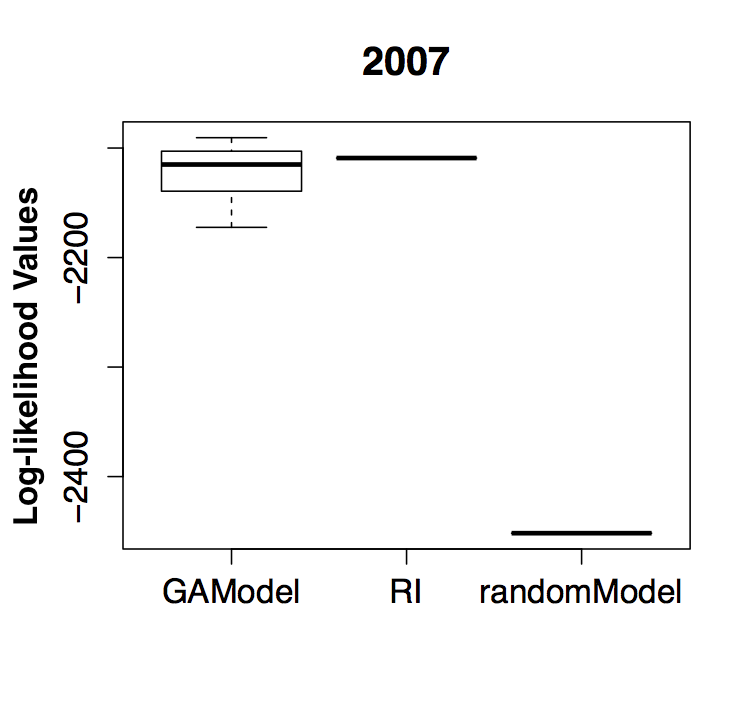
\includegraphics[scale=0.55]{boxPlot2007.png}
		\caption{Box-plot of the values obtained by the models for the year 2007.}
		\label{boxPlot2007}
	\end{minipage}\hfill
	\begin{minipage}{0.45\textwidth}
		\centering
		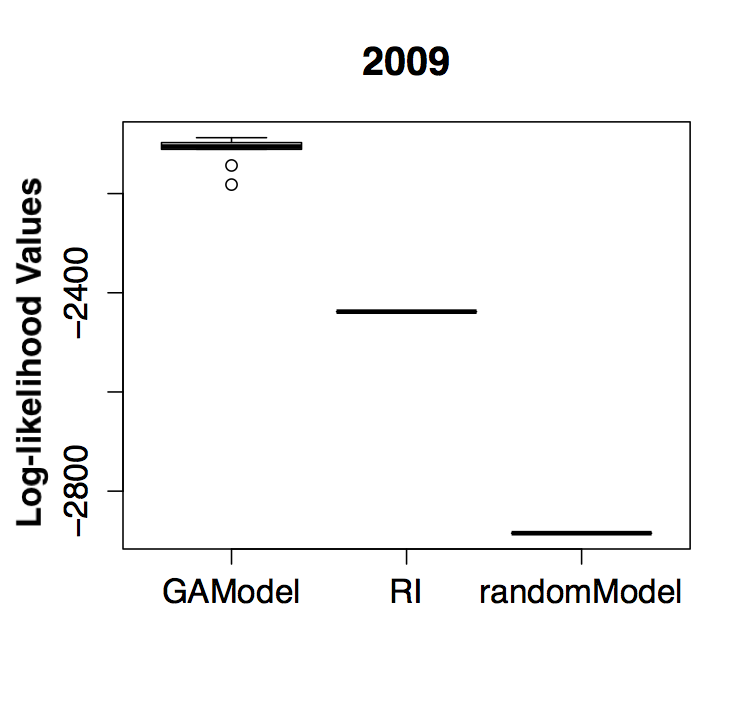
\includegraphics[scale=0.55]{boxPlot2009.png}
		\caption{Box-plot of the values obtained by the models for the year 2009.}
		\label{boxPlot2009}
	\end{minipage}
\end{figure}

\subsection{Models Example and The Real Data}

The Figure~\ref{modeloGAModel} shows a model from the GAModel method for the year 2010. It indicates a low earthquake intensity as green while the more intensity areas, are shown as orange (for even higher cases, white is used). The Figure~\ref{modeloRI} shows a model from the RI Algorithm for the year 2010. It indicates a low earthquake intensity as white while the more intensity areas, are shown in red. For comparison reasons, we show the Figure~\ref{realData}, that shows the earthquake occurrences for the same year.\\


\begin{figure}[H]
	\centering
	\begin{minipage}{0.45\textwidth}
		\centering
		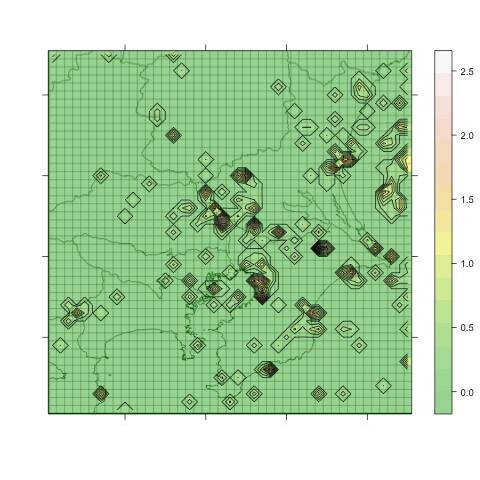
\includegraphics[scale=0.4]{media2010.jpg}
		\caption{ GAModel model for the year of 2010 in Kanto.}
		\label{modeloGAModel}
	\end{minipage}\hfill
	\begin{minipage}{0.45\textwidth}
		\centering
			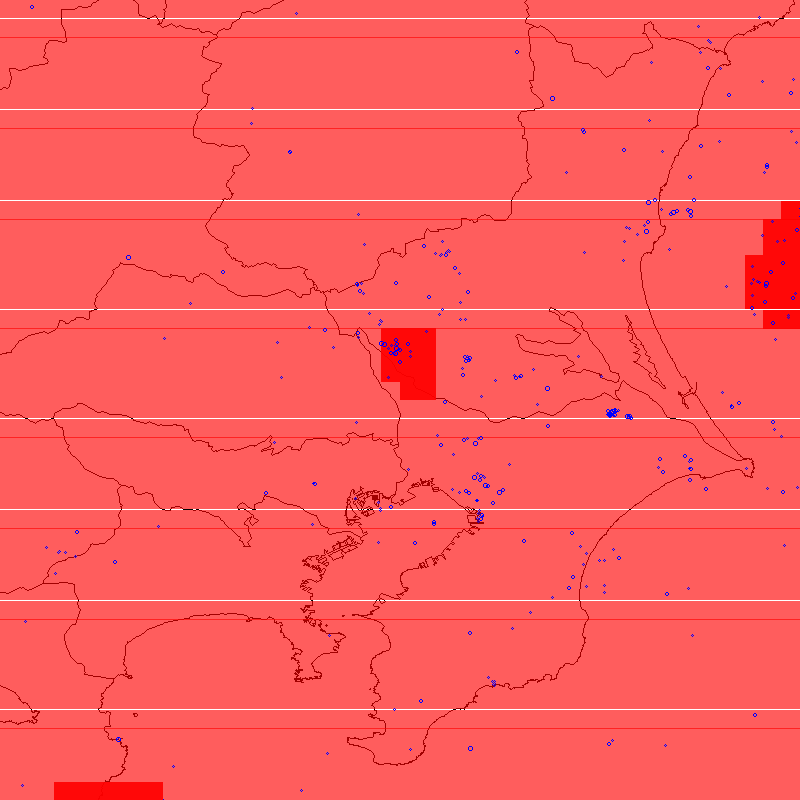
\includegraphics[scale=0.18]{kanto10_RI.png}
			\caption{RI model for the year of 2010 in Kanto. Figure from~\cite{ecta14}.}
			\label{modeloRI}
	\end{minipage}
	\begin{minipage}{0.45\textwidth}
		\centering
		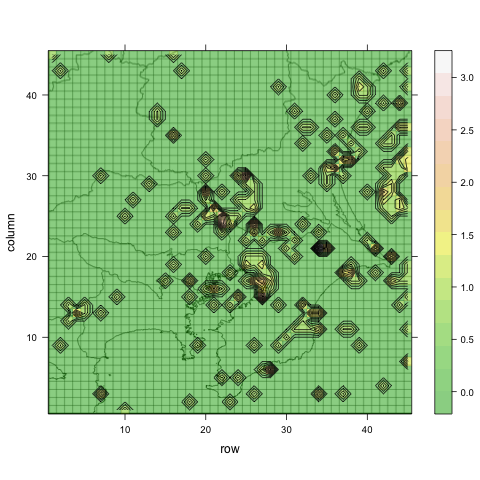
\includegraphics[scale=0.4]{matriz2010_real.png}
		\caption{Earthquake occurrences in the year of 2010 in Kanto}
		\label{realData}
	\end{minipage}
\end{figure}


\section{Results from The Main-shock Models Main-shock with After-shock Models Experiment}
A one-way between subjects ANOVA was conducted to compare the effects of the models, the depths, the years and regions on the log-likelihood value. In this study there are 6 options for model: ReducedGAModel, GAModel, Emp-GAModel, Emp-ReducedGAModel, GAModelClustered and ReducedGAModelClustered. \\

For all, the confidence interval is set to 5\%.\\

Based on the results of the test, there was a not a significant effect of the depths or years variables. For both cases at the we obtaind p>0.05 level for the depths condition [F(2) = 2.072, p = 0.126] and we also obtained p>0.05 for the years condition  [F(5) = 0.050, p = 0.999]. There was a significant effect of the models condition (p>0.05 [F(5) = 9699.690, p<2e-16]) and regions condition (p>0.05 [F(3) = 764.220, p<2e-16]). Therefore, we conduct a new ANOVA test, with only the last two variables to verify the influence of those conditions more accurately. The results only changed a little, maintaining the significant effect of both conditions, p>0.05 [F(5) = 9705.6, p<2e-16] and p>0.05 [F(3) = 764.7, p <2e-16], respectively.\\

The results of the experiments are in the Table~\ref{anovatest}. 

The column labelled Random shows the result of the RandomModel, and the idea the is same for the ones labelled GAModel and RI. The ``p-value'' shows significance value of the {\it Student's t-test} for null hypothesis `` The mean of the log-likelihood values is greater that the values for RI''.\\

\begin{table*}[!ht]
	\centering
	\begin{tabular}{|l|l|l|l|l|l|}
		\hline
		{Variable} & {Degrees of Freedom} & {Sum Sq}    & {Mean Sq}   & {F Value} & {Pr(\textgreater F)} \\
		\hline
		Model    & 31424058           & 6284812   & 6284812   & 255.0   & \textless2e-16     \\
		\hline
		Depth    & 2                  & 16077491  & 8038746   & 326.2   & \textless2e-16     \\
		\hline
		Year     & 5                  & 57908014  & 11581603  & 470.0   & \textless2e-16     \\
		\hline
		Region   & 3                  & 878253346 & 292751115 & 11879.4 & \textless2e-16\\    
		\hline
	\end{tabular}
	\caption{Simple ANOVA Test Results.}
	\label{anovatest}
\end{table*}

Because we found statistically significant result, we applied a Post hoc comparisons using the Tukey HSD test. It compared each condition with all others. For example, it compares the values from the GAModel with the GAModelClustered, see~\ref{modelANOVA}. It indicated that the GAModelClustered and ReducedGAModelClustered, when compared with all other models, achieve greater log-likelihood values. Furthermore, we noticed that the depths conditions show a greater influence when the depth in smaller or equal to 25 km, see Figure~\ref{depthsANOVA}.\\

\begin{figure}[H]
	\centering
	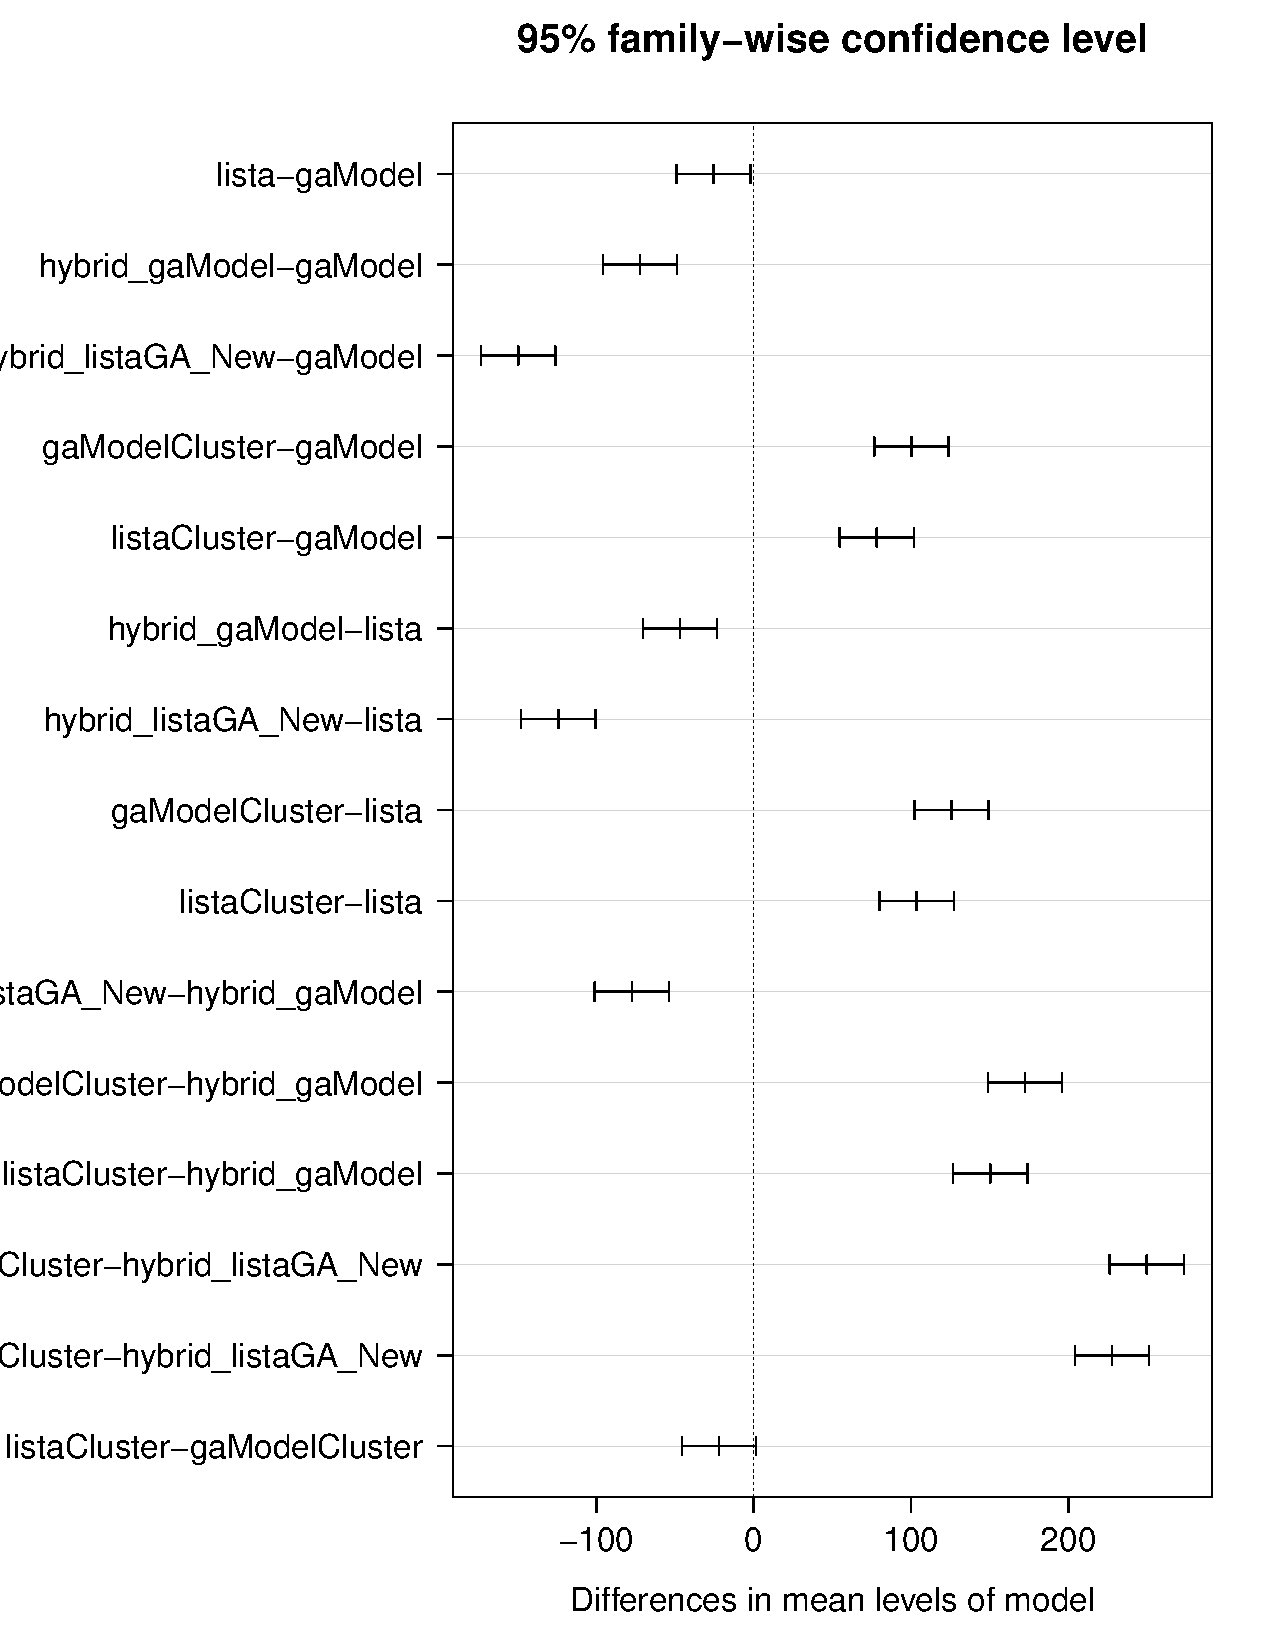
\includegraphics[scale=0.45]{modelANOVA.pdf}
	\caption{ANOVA results - Models.}
	\label{modelANOVA}
\end{figure}

\begin{figure}[H]
	\centering
	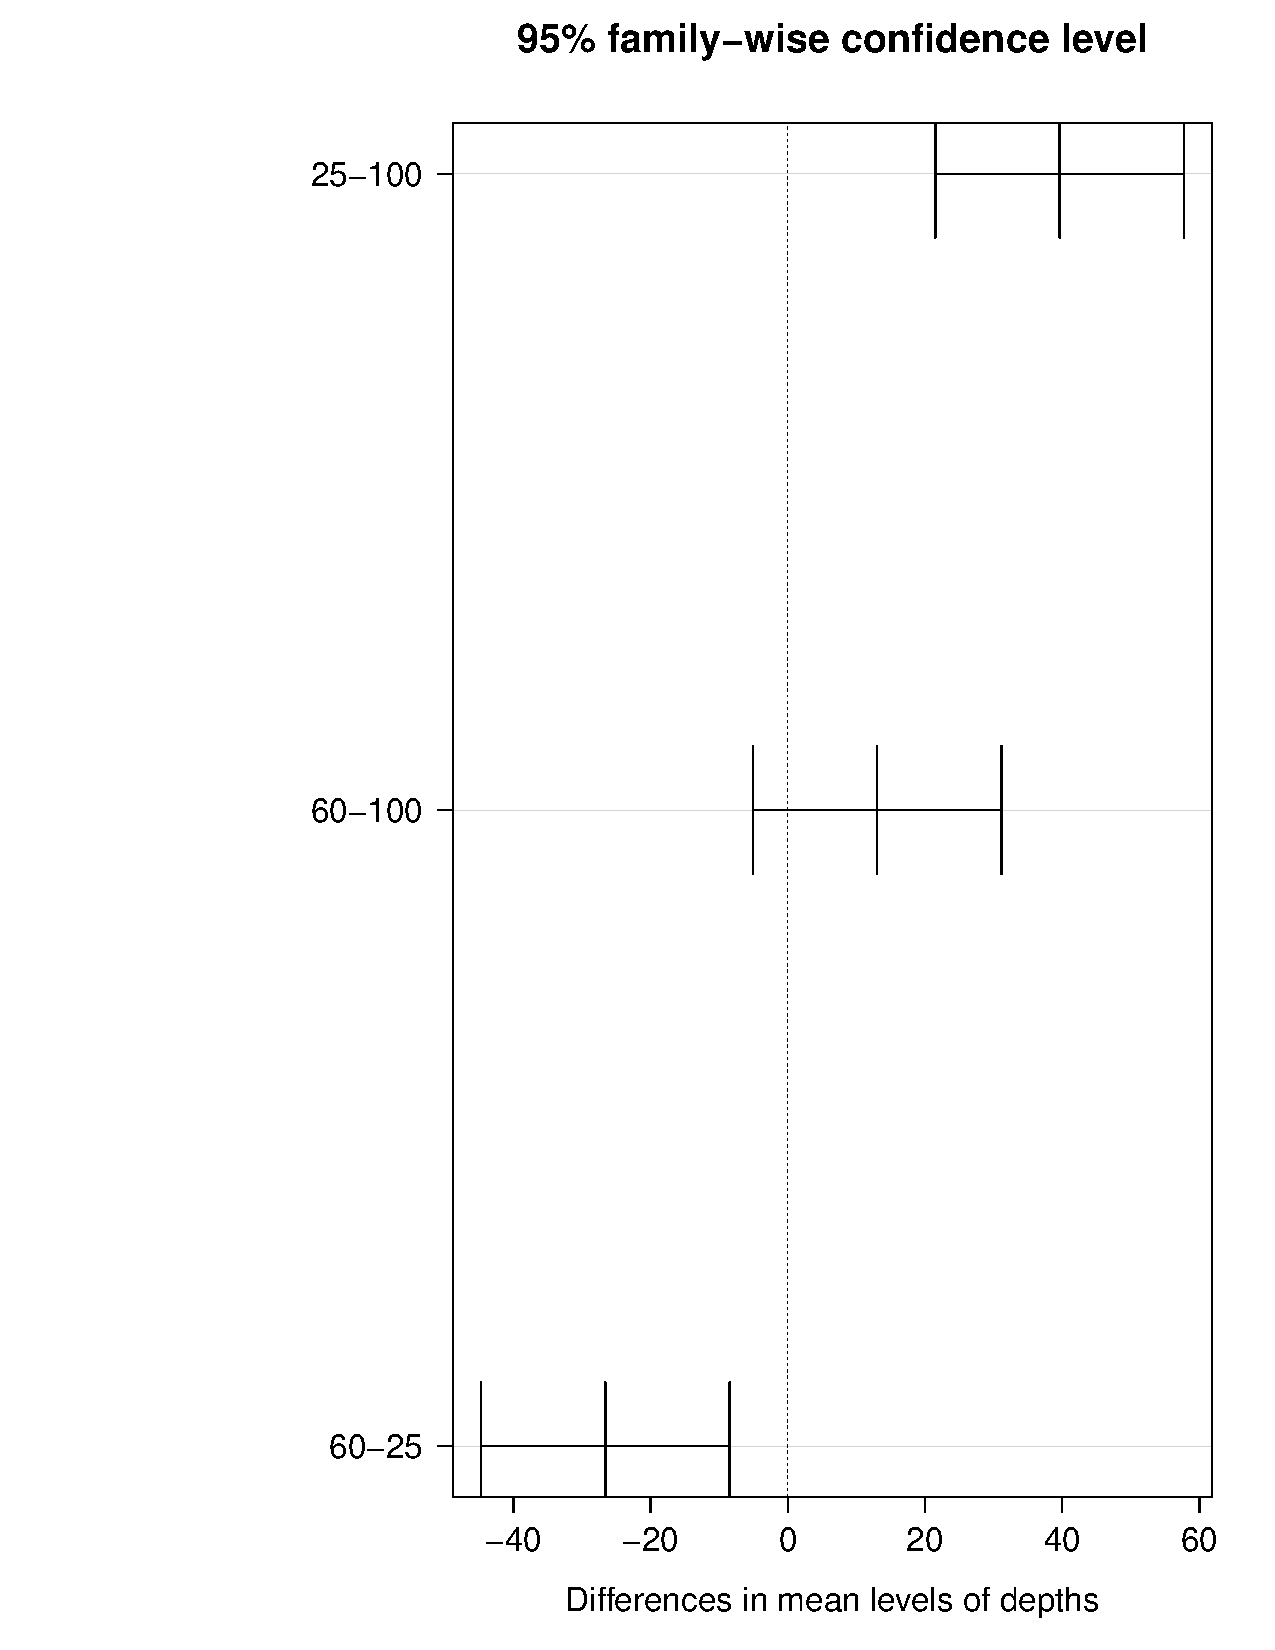
\includegraphics[scale=0.45]{depthsClusterANOVA.pdf}
	\caption{ANOVA results - Depths.}
	\label{depthsANOVA}
\end{figure}

When comparing the models from the ReducedGAModel and from the GAModel against themselves, with or without using clustering catalogues, we found that there is no statistically significant result between the methods. That implies it can be considered that the methods are obtain statistically equal results.\\

Therefore, based on the result of HSD test, we performed a new ANOVA test, considering only the GAModelClustered and the ReducedGAModelClustered That was meant not only to verify the previous results but also to certify if the depth influence is preserved.\\

\begin{table*}[!ht]
	\centering
	\begin{tabular}{|l|l|l|l|l|l|}
		\hline
		{Variable} & {Degrees of Freedom} & {Sum Sq}    & {Mean Sq}   & {F Value} & {Pr(\textgreater F)} \\
		\hline
		Model    & 1           & 174862   & 174862   & 12.22   & \textless0.000488     \\
		\hline
		
		Depth    & 2                  & 391370  & 195685   & 13.67   & \textless1.32e-06     \\
		\hline
		Year     & 5                  & 18810831  & 3762166  & 262.82   & \textless2e-16     \\
		\hline
		Region   & 3                  & 249741769 & 83247256 & 5815.53 & \textless2e-16\\    
		\hline
	\end{tabular}
	\caption{ANOVA Test Results - Only Clustered Data.}
	\label{newanovatest}
\end{table*}


Taken together, these results suggest that the using cluster and depth smaller or equal to 25km, see Figure~\ref{depthsClusterANOVA} showed the best results.\\

\begin{figure}[H]
	\centering
	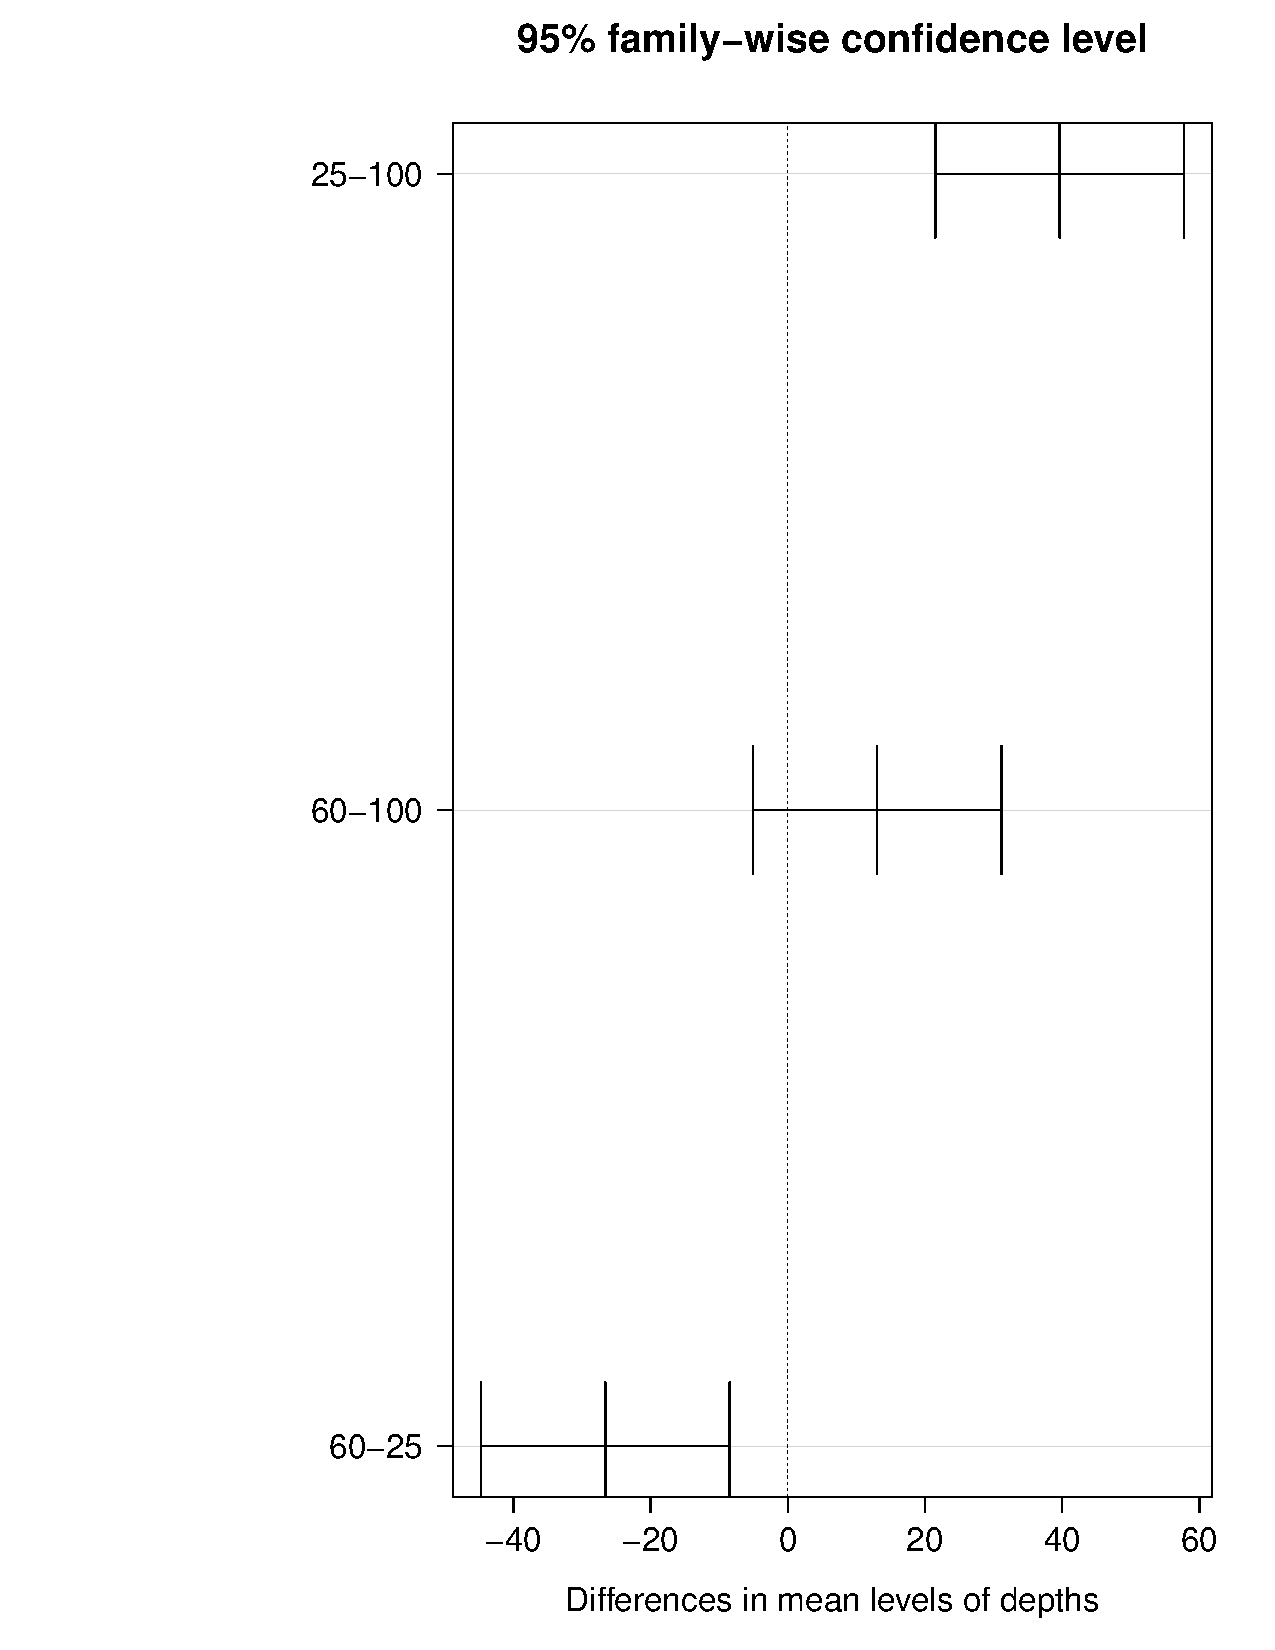
\includegraphics[scale=0.45]{depthsClusterANOVA.pdf}
	\caption{Second ANOVA results - Depths.}
	\label{depthsClusterANOVA}
\end{figure}

\subsection{The Models Examples And The Real Data}

The Figure~\ref{gamodel2005eastjapan} shows a model from the GAModel method for the year 2005 in East Japan. The next Figure,~\ref{reduced2005eastjapan} shows a model from the ReducedGAModel~\ref{reducedGAModel} method for the year 2005 in East Japan.\\

All Figures,~\ref{gamodel2005eastjapan}~\ref{reduced2005eastjapan}~\ref{hybridgamodel2005eastjapan}~\ref{hybridreduced2005eastjapan},  indicate a low earthquake intensity as white while the more intensity areas, are shown in red. They are, in order, the data visualisation for the model from: the GAModel, the ReducedGAModel, the Emp-GAModel and the Emp-ReducedGAModel for East Japan in 2005. The Figure~\ref{real2005eastjapan} represents the earthquake occurrences in the same region and year.\\


\begin{figure}[H]
	\centering
	\begin{minipage}{0.45\textwidth}
		\centering
		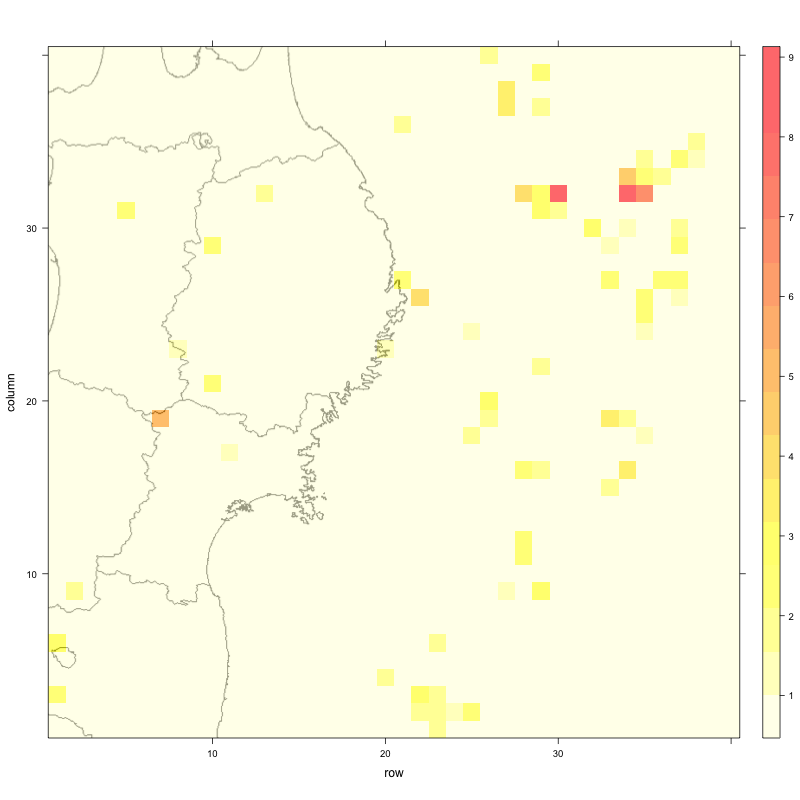
\includegraphics[scale=0.2]{gamodel2005eastjapan.png}
		\caption{GAModel model for the year of 2005 in East Japan.}
		\label{gamodel2005eastjapan}
	\end{minipage}
	\begin{minipage}{0.45\textwidth}

	\end{minipage}
\end{figure}


\begin{figure}[H]
	\centering
	\begin{minipage}{0.45\textwidth}
		\centering
		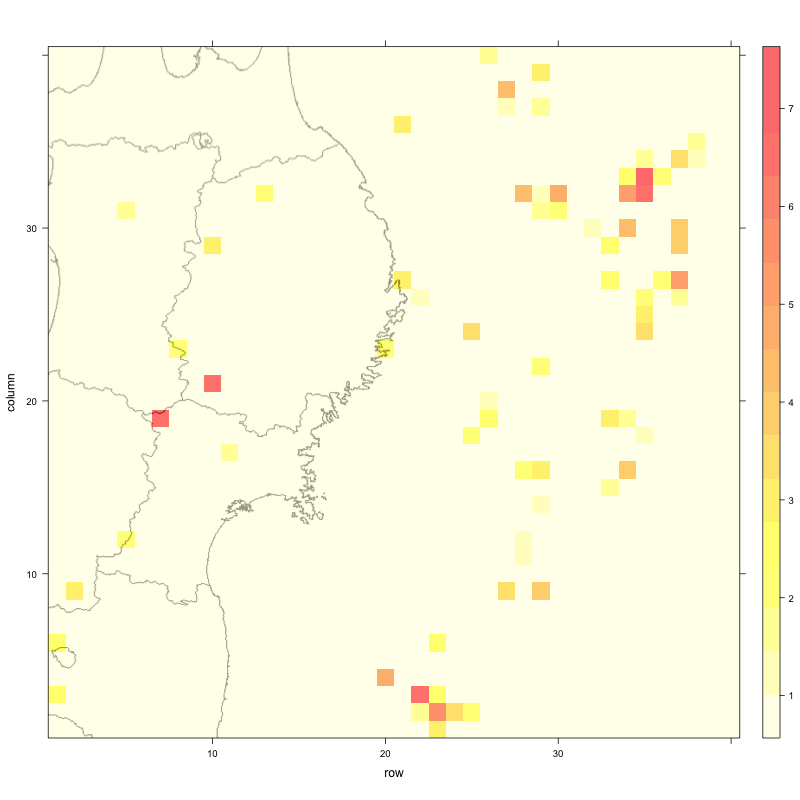
\includegraphics[scale=0.2]{reduced2005eastjapan.png}
		\caption{ReducedGAModel model for the year of 2005 in East Japan.}
		\label{reduced2005eastjapan}
	\end{minipage}
	\begin{minipage}{0.45\textwidth}
		\centering
		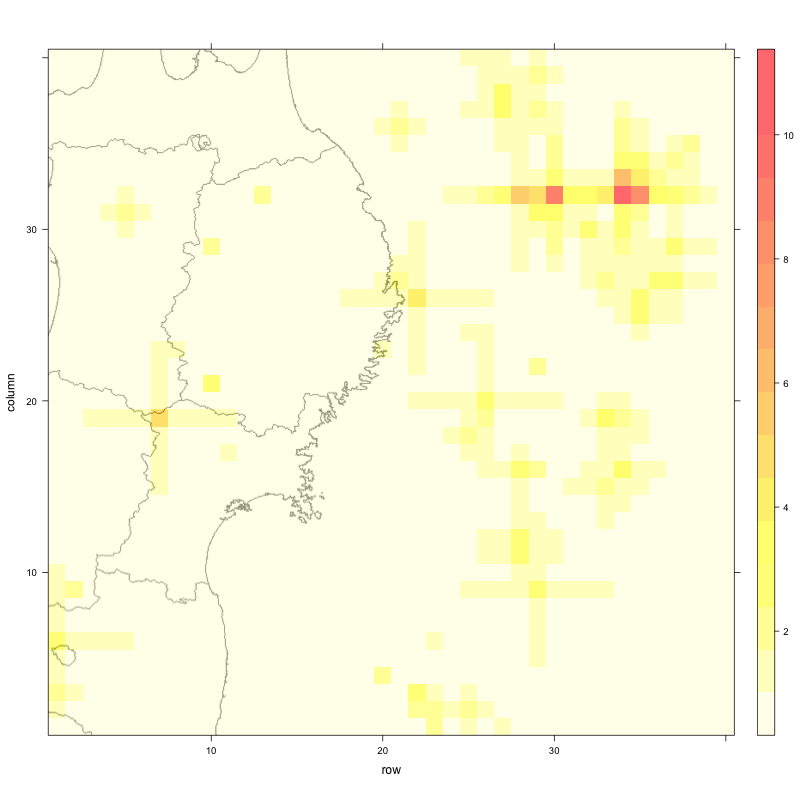
\includegraphics[scale=0.2]{hybridgamodel2005eastjapan.png}
		\caption{Em-GAModel model for the year of 2005 in East Japan.}
		\label{hybridgamodel2005eastjapan}
	\end{minipage}
\end{figure}

\begin{figure}[H]
	\begin{minipage}{0.45\textwidth}
		\centering
			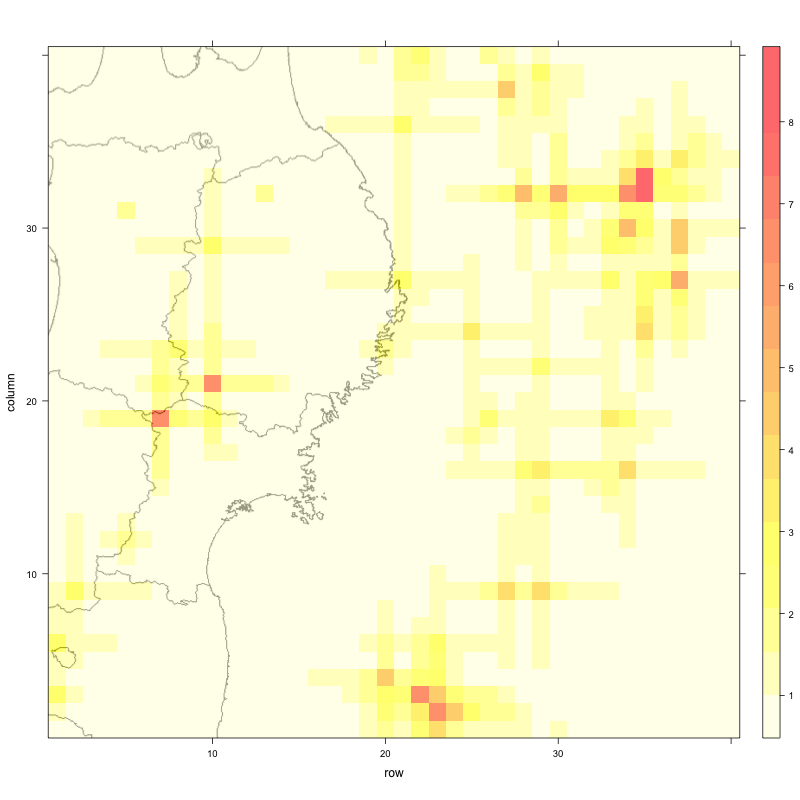
\includegraphics[scale=0.2]{hybridreduced2005eastjapan.png}
			\caption{Emp-ReducedGAModel model for the year of 2005 in East Japan.}
			\label{hybridreduced2005eastjapan}
	\end{minipage}
	\begin{minipage}{0.45\textwidth}
		\centering
		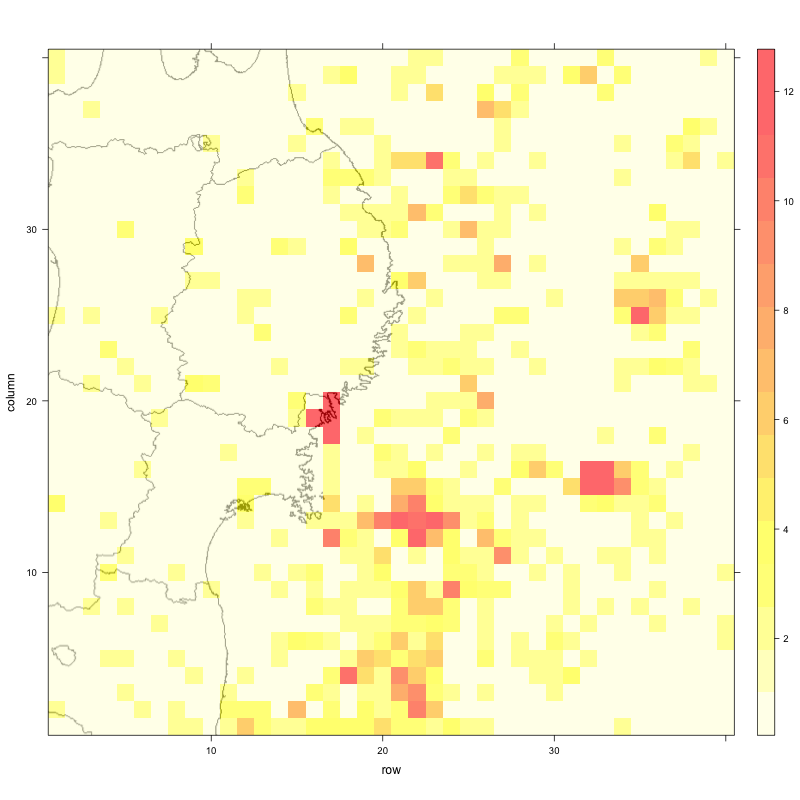
\includegraphics[scale=0.2]{real2005eastjapan.png}
		\caption{Earthquake occurrences in the year of 2005 in East Japan.}
		\label{real2005eastjapan}
	\end{minipage}
\end{figure}


\subsection{Paired Design}

To further explore the only the variations from the models on the regions, disregarding any other variable, we applied an paired Student’s t-test. 
%TODO: tem que fazer isso pra kanto, kansai, touhoku e EastJapan?
\begin{table*}[!ht]
	\begin{center}
		\begin{tabular}{|l|l|c|cc|c|}
			\hline
			\multicolumn{1}{|c|}{Scenario} & \multicolumn{5}{|c|}{Log Likelihood} \\
			\hline
			\multicolumn{1}{|c|}{Year} & \multicolumn{1}{|c|}{Random} & \multicolumn{1}{|c|}{RI} & \multicolumn{2}{c}{GAModel} & \multicolumn{1}{|c|}{p-value} \\    
			\hline
			2000 &-2413.89 &-2124.44 &\raggedright  -2094.05 &\raggedleft (8.80) & 0.01\\%better
			2001 &-2418.14 &-2103.19 &\raggedright  -2101.65 &\raggedleft  (69.49) & 0.57\\%equal
			2002 &-2385.04 &-2094.43 &\raggedright  -2100.01 &\raggedleft (72.62) & 0.07\\%equal
			2003 &-2401.00 &-2104.65 &\raggedright  -2100.76 &\raggedleft (156) & 0.35\\%equal
			2004 &-2421.92 &-2101.92 &\raggedright  -2098.30 &\raggedleft (55.28) & 0.16\\%equal
			2005 &-2643.38 &-2248.40 &\raggedright  -2114.00 &\raggedleft (779) & 0.01\\%better
			2006 &-2616.50 &-2226.93 &\raggedright  -2115.6 &\raggedleft (633) & 0.01\\%better
			2007 &-2451.68 &-2109.13 &\raggedright  -2122.03 &\raggedleft (615) &  0.13\\%equal
			2008 &-2433.23 &-2112.92 &\raggedright  -4435.34 &\raggedleft (657) & 0.14\\%equal
			2009 &-2884.74 &-2438.10 &\raggedright  -2113.1 &\raggedleft (814) & 0.01\\%better
			2010 &-2418.18 &-2114.60 &\raggedright -2112.07 &\raggedleft (843) & 0.79\\%equal
			\hline
		\end{tabular}
	\end{center}
	\caption{Experiments result - Paired Design.}
	\label{gaxriTable??}
\end{table*}